% Options for packages loaded elsewhere
\PassOptionsToPackage{unicode}{hyperref}
\PassOptionsToPackage{hyphens}{url}
\PassOptionsToPackage{dvipsnames,svgnames,x11names}{xcolor}
%
\documentclass[
  letterpaper,
  DIV=11,
  numbers=noendperiod]{scrartcl}

\usepackage{amsmath,amssymb}
\usepackage{iftex}
\ifPDFTeX
  \usepackage[T1]{fontenc}
  \usepackage[utf8]{inputenc}
  \usepackage{textcomp} % provide euro and other symbols
\else % if luatex or xetex
  \usepackage{unicode-math}
  \defaultfontfeatures{Scale=MatchLowercase}
  \defaultfontfeatures[\rmfamily]{Ligatures=TeX,Scale=1}
\fi
\usepackage{lmodern}
\ifPDFTeX\else  
    % xetex/luatex font selection
\fi
% Use upquote if available, for straight quotes in verbatim environments
\IfFileExists{upquote.sty}{\usepackage{upquote}}{}
\IfFileExists{microtype.sty}{% use microtype if available
  \usepackage[]{microtype}
  \UseMicrotypeSet[protrusion]{basicmath} % disable protrusion for tt fonts
}{}
\makeatletter
\@ifundefined{KOMAClassName}{% if non-KOMA class
  \IfFileExists{parskip.sty}{%
    \usepackage{parskip}
  }{% else
    \setlength{\parindent}{0pt}
    \setlength{\parskip}{6pt plus 2pt minus 1pt}}
}{% if KOMA class
  \KOMAoptions{parskip=half}}
\makeatother
\usepackage{xcolor}
\setlength{\emergencystretch}{3em} % prevent overfull lines
\setcounter{secnumdepth}{5}
% Make \paragraph and \subparagraph free-standing
\makeatletter
\ifx\paragraph\undefined\else
  \let\oldparagraph\paragraph
  \renewcommand{\paragraph}{
    \@ifstar
      \xxxParagraphStar
      \xxxParagraphNoStar
  }
  \newcommand{\xxxParagraphStar}[1]{\oldparagraph*{#1}\mbox{}}
  \newcommand{\xxxParagraphNoStar}[1]{\oldparagraph{#1}\mbox{}}
\fi
\ifx\subparagraph\undefined\else
  \let\oldsubparagraph\subparagraph
  \renewcommand{\subparagraph}{
    \@ifstar
      \xxxSubParagraphStar
      \xxxSubParagraphNoStar
  }
  \newcommand{\xxxSubParagraphStar}[1]{\oldsubparagraph*{#1}\mbox{}}
  \newcommand{\xxxSubParagraphNoStar}[1]{\oldsubparagraph{#1}\mbox{}}
\fi
\makeatother


\providecommand{\tightlist}{%
  \setlength{\itemsep}{0pt}\setlength{\parskip}{0pt}}\usepackage{longtable,booktabs,array}
\usepackage{calc} % for calculating minipage widths
% Correct order of tables after \paragraph or \subparagraph
\usepackage{etoolbox}
\makeatletter
\patchcmd\longtable{\par}{\if@noskipsec\mbox{}\fi\par}{}{}
\makeatother
% Allow footnotes in longtable head/foot
\IfFileExists{footnotehyper.sty}{\usepackage{footnotehyper}}{\usepackage{footnote}}
\makesavenoteenv{longtable}
\usepackage{graphicx}
\makeatletter
\def\maxwidth{\ifdim\Gin@nat@width>\linewidth\linewidth\else\Gin@nat@width\fi}
\def\maxheight{\ifdim\Gin@nat@height>\textheight\textheight\else\Gin@nat@height\fi}
\makeatother
% Scale images if necessary, so that they will not overflow the page
% margins by default, and it is still possible to overwrite the defaults
% using explicit options in \includegraphics[width, height, ...]{}
\setkeys{Gin}{width=\maxwidth,height=\maxheight,keepaspectratio}
% Set default figure placement to htbp
\makeatletter
\def\fps@figure{htbp}
\makeatother
% definitions for citeproc citations
\NewDocumentCommand\citeproctext{}{}
\NewDocumentCommand\citeproc{mm}{%
  \begingroup\def\citeproctext{#2}\cite{#1}\endgroup}
\makeatletter
 % allow citations to break across lines
 \let\@cite@ofmt\@firstofone
 % avoid brackets around text for \cite:
 \def\@biblabel#1{}
 \def\@cite#1#2{{#1\if@tempswa , #2\fi}}
\makeatother
\newlength{\cslhangindent}
\setlength{\cslhangindent}{1.5em}
\newlength{\csllabelwidth}
\setlength{\csllabelwidth}{3em}
\newenvironment{CSLReferences}[2] % #1 hanging-indent, #2 entry-spacing
 {\begin{list}{}{%
  \setlength{\itemindent}{0pt}
  \setlength{\leftmargin}{0pt}
  \setlength{\parsep}{0pt}
  % turn on hanging indent if param 1 is 1
  \ifodd #1
   \setlength{\leftmargin}{\cslhangindent}
   \setlength{\itemindent}{-1\cslhangindent}
  \fi
  % set entry spacing
  \setlength{\itemsep}{#2\baselineskip}}}
 {\end{list}}
\usepackage{calc}
\newcommand{\CSLBlock}[1]{\hfill\break\parbox[t]{\linewidth}{\strut\ignorespaces#1\strut}}
\newcommand{\CSLLeftMargin}[1]{\parbox[t]{\csllabelwidth}{\strut#1\strut}}
\newcommand{\CSLRightInline}[1]{\parbox[t]{\linewidth - \csllabelwidth}{\strut#1\strut}}
\newcommand{\CSLIndent}[1]{\hspace{\cslhangindent}#1}

\KOMAoption{captions}{tableheading}
\makeatletter
\@ifpackageloaded{caption}{}{\usepackage{caption}}
\AtBeginDocument{%
\ifdefined\contentsname
  \renewcommand*\contentsname{Table of contents}
\else
  \newcommand\contentsname{Table of contents}
\fi
\ifdefined\listfigurename
  \renewcommand*\listfigurename{List of Figures}
\else
  \newcommand\listfigurename{List of Figures}
\fi
\ifdefined\listtablename
  \renewcommand*\listtablename{List of Tables}
\else
  \newcommand\listtablename{List of Tables}
\fi
\ifdefined\figurename
  \renewcommand*\figurename{Figure}
\else
  \newcommand\figurename{Figure}
\fi
\ifdefined\tablename
  \renewcommand*\tablename{Table}
\else
  \newcommand\tablename{Table}
\fi
}
\@ifpackageloaded{float}{}{\usepackage{float}}
\floatstyle{ruled}
\@ifundefined{c@chapter}{\newfloat{codelisting}{h}{lop}}{\newfloat{codelisting}{h}{lop}[chapter]}
\floatname{codelisting}{Listing}
\newcommand*\listoflistings{\listof{codelisting}{List of Listings}}
\makeatother
\makeatletter
\makeatother
\makeatletter
\@ifpackageloaded{caption}{}{\usepackage{caption}}
\@ifpackageloaded{subcaption}{}{\usepackage{subcaption}}
\makeatother
\ifLuaTeX
  \usepackage{selnolig}  % disable illegal ligatures
\fi
\usepackage{bookmark}

\IfFileExists{xurl.sty}{\usepackage{xurl}}{} % add URL line breaks if available
\urlstyle{same} % disable monospaced font for URLs
\hypersetup{
  pdftitle={T is for Topology},
  pdfauthor={Tanya Strydom; Jennifer A. Dunne; Timothée Poisot; Andrew P. Beckerman},
  pdfkeywords={food web, network construction},
  colorlinks=true,
  linkcolor={blue},
  filecolor={Maroon},
  citecolor={Blue},
  urlcolor={Blue},
  pdfcreator={LaTeX via pandoc}}

\title{T is for Topology}
\author{Tanya Strydom \and Jennifer A. Dunne \and Timothée
Poisot \and Andrew P. Beckerman}
\date{2024-04-19}

\begin{document}
\maketitle
\begin{abstract}
There are many reasons one might want to generate a network and there
are many tools on the market that might make that possible. However not
all tools are created equally and there is reason to assume that not all
networks will suit most purposes. Here the aim is to compare and
contrast the different topology generating tools that are on the market
and see where they shine and where they fall flat. There probably isn't
one model to rule them all but it doesn't mean that we shouldn't be
critical when we think about the model we want to use.
\end{abstract}

\section{Introduction}\label{introduction}

\begin{itemize}
\item
  In order to construct a `perfect' network \emph{i.e.,} one which
  \emph{perfectly} captures the dynamics for a specific community at a
  specific time one needs to consider and account for many different
  moving parts (\emph{e.g.,}). So when developing a model it makes sense
  that you prioritise the aspect of the prediction/construction task
  that has the most value for your research goal, acknowledging that a
  model might fall short in others. The thing is that with the growing
  suite of approaches to generating networks it is important that we
  don't lose sight of the core philosophy behind the model we use and to
  ensure that we are using the model best suited to what we want to be
  accomplishing.

  \begin{itemize}
  \tightlist
  \item
    Bring up the fact that delimiting a network is in and of itself
    fuzzy - we tend to think of them in terms of snapshots but in
    reality the final (empirical) network is often the result of
    aggregation over multiple timescales.
  \item
    Also the fact that \emph{some} people are concerned about the
    taxonomic resolution and cascading effects those might have on our
    understanding of network structure (Pringle and Hutchinson 2020;
    Pringle 2020), we are at risk of losing our ability to distinguish
    the wood from the tree - are we not (at least at times) concerned
    more with understanding ecosystem level processes than with needing
    to understand things \emph{perfectly} at the species level.
  \end{itemize}
\item
  What do we mean when we talk about an `interaction network'? Is it the
  flow of biomass/energy? Is it an effect on fitness (feeding)? (can we
  really represent indirect interactions as actual links?)

  \begin{itemize}
  \tightlist
  \item
    ``For example, nodes can be individuals and the links contacts
    between those individuals (Melian et al.~2011), nodes can be species
    and the links the interactions (e.g.~feeding, mutualistic,
    parasitic) between them (de Ruiter et al.~1995), or nodes can be
    ecological communities or ecosystems and the links fluxes between
    these localities (Proulx et al.~2005; Chadès et al.~2011)'' -
    Poisot, Stouffer, and Kéfi (2016)
  \end{itemize}
\item
  It is perhaps useful to start with asking why do we want/need models
  to generate networks. This can be broadly thought of to fall into two
  categories. Build networks because we want to build concepts vs build
  networks because we want specificity. Broadly this means that we
  either want to construct/predict a collection of interactions
  (generate networks) or a network of interactions (predict
  interactions).

  \begin{itemize}
  \tightlist
  \item
    ``For example, dynamic models focus on how structure relates to
    population dynamics and community stability (2, 7--11). Evolutionary
    models incorporate the processes that control the formation and
    expansion of food webs (12, 13). Static models include rules that
    determine structural attributes of food webs (14--19).'' - Petchey
    et al. (2008)
  \end{itemize}
\end{itemize}

Arguably the need for methods and tools for constructing interaction
networks arises from two different (but still aligned) places of
interest within the field of network ecology. On the one side sits the
researcher who is interested in generating a set of ecologically
plausible networks for the purpose of running further simulations
(\emph{e.g.,} extinction simulations) or understanding some higher-level
process/concept (\emph{e.g.,} understanding energy flows), importantly
these networks do not require any level of species specificity \emph{per
se} and it is more the arrangements of the nodes (species) within the
context of network structure that is of value. This researcher is
contrasted by one that is interested in constructing real-world,
location specific, interaction data for a specific collection of species
(community). This is driven by the need for researchers to find
alternative ways to infer the interactions between species as a way to
overcome the inherit challenges of inventorying interaction in the field
(Morales-Castilla et al. 2015; Strydom et al. 2021). Of course these two
categories are not distinct, mutually exclusive, groups but can rather
be viewed as operating on a gradient ranging from a need for generality
(\emph{i.e.,} creating a network that, when taken in aggregate, the
distribution of links (interactions) between species are ecologically
plausible) to a need for specificity (\emph{i.e.,} local-level
predictions between specific species).

\begin{itemize}
\item
  Brief history of the development of tools within the context of the
  two different fields? Sort of where the theory/body of work was based
  and how that has changed?

  \begin{itemize}
  \item
    Core mechanistic differences that models will work at --- some are
    really concerned about (and thus constrained by) structure, others
    are more mechanistic in nature \emph{i.e.,} species \emph{a} has the
    capacity to eat species \emph{b} because traits
  \item
    In certain situations structure is `enough' but there may be use
    cases where we are really interested in the node-level interactions
    \emph{i.e.,} species identity is a thing we care about and need to
    be able to retrieve specific interactions at specific nodes
    correctly.
  \item
    What is the purpose of generating a network? Is it an element of a
    bigger question we are asking, \emph{e.g.,} I want to generate a
    series of networks to do some extinction simulations/bioenergetic
    stuff OR are we looking for a `final product' network that is
    relevant to a specific location? (this can still be broad in
    geographic scope).
  \end{itemize}
\item
  A breakdown of wanting to generate a network; statement of need and
  core philosophies
\item
  A breakdown of wanting to predict an interaction; statement of need
  (Jordano 2016b, 2016a; Poisot et al. 2021) and core philosophies
  (trait-matching, coexistence, evolutionary backbones)
\item
  Stands to reason then that we have developed methods that specialise
  in one or the other. Which comes at a cost of `performance' in other
  aspects. Knowing how the different model families stack up to each
  other is thus valuable.
\end{itemize}

Joel E. Cohen, Newman, and Steele (1985) states that \emph{``{[}Their{]}
approach is more like gross anatomy than like physiology\ldots{} that
is, the gross anatomy is frozen, rather than in motion.''}.

Interestingly Williams and Martinez (2008) also explicitly talk about
\emph{structural} food-web models in their introduction\ldots{} so how I
see it that means that there has always been this inherent
acknowledgement that models are functioning at a specific `network
level'.

Other works to keep in mind: Pringle and Hutchinson (2020), Pringle
(2020)

\begin{quote}
``The resolution of food-web data is demonic because it can radically
change network topology and associated biological inferences in ways
that are unknowable in the absence of better data.'' - Pringle and
Hutchinson (2020)
\end{quote}

\begin{quote}
``It makes no sense to describe the interaction structure of nodes which
in themselves are poorly defined.'' --- Roslin et al.~(2013, p.~2)
\end{quote}

\section{Model families}\label{model-families}

Given the large number of models that have been developed it is perhaps
more meaningful to group models into families with the idea that models
from the same family will yield similar results because they play by
similar rules. These rules referring to the underlying philosophy as to
what structures either networks or the interactions within them (see
Figure~\ref{fig-concept} panel A). Although there have been efforts to
compare and contrast different models (\emph{e.g.,} Williams and
Martinez 2008 looked at `structural' models; and Pichler et al. 2020
looked at `machine learning algorithms') there still lacks an overall
synthesis as to how the different model families differ from each other.

\begin{figure}

\centering{

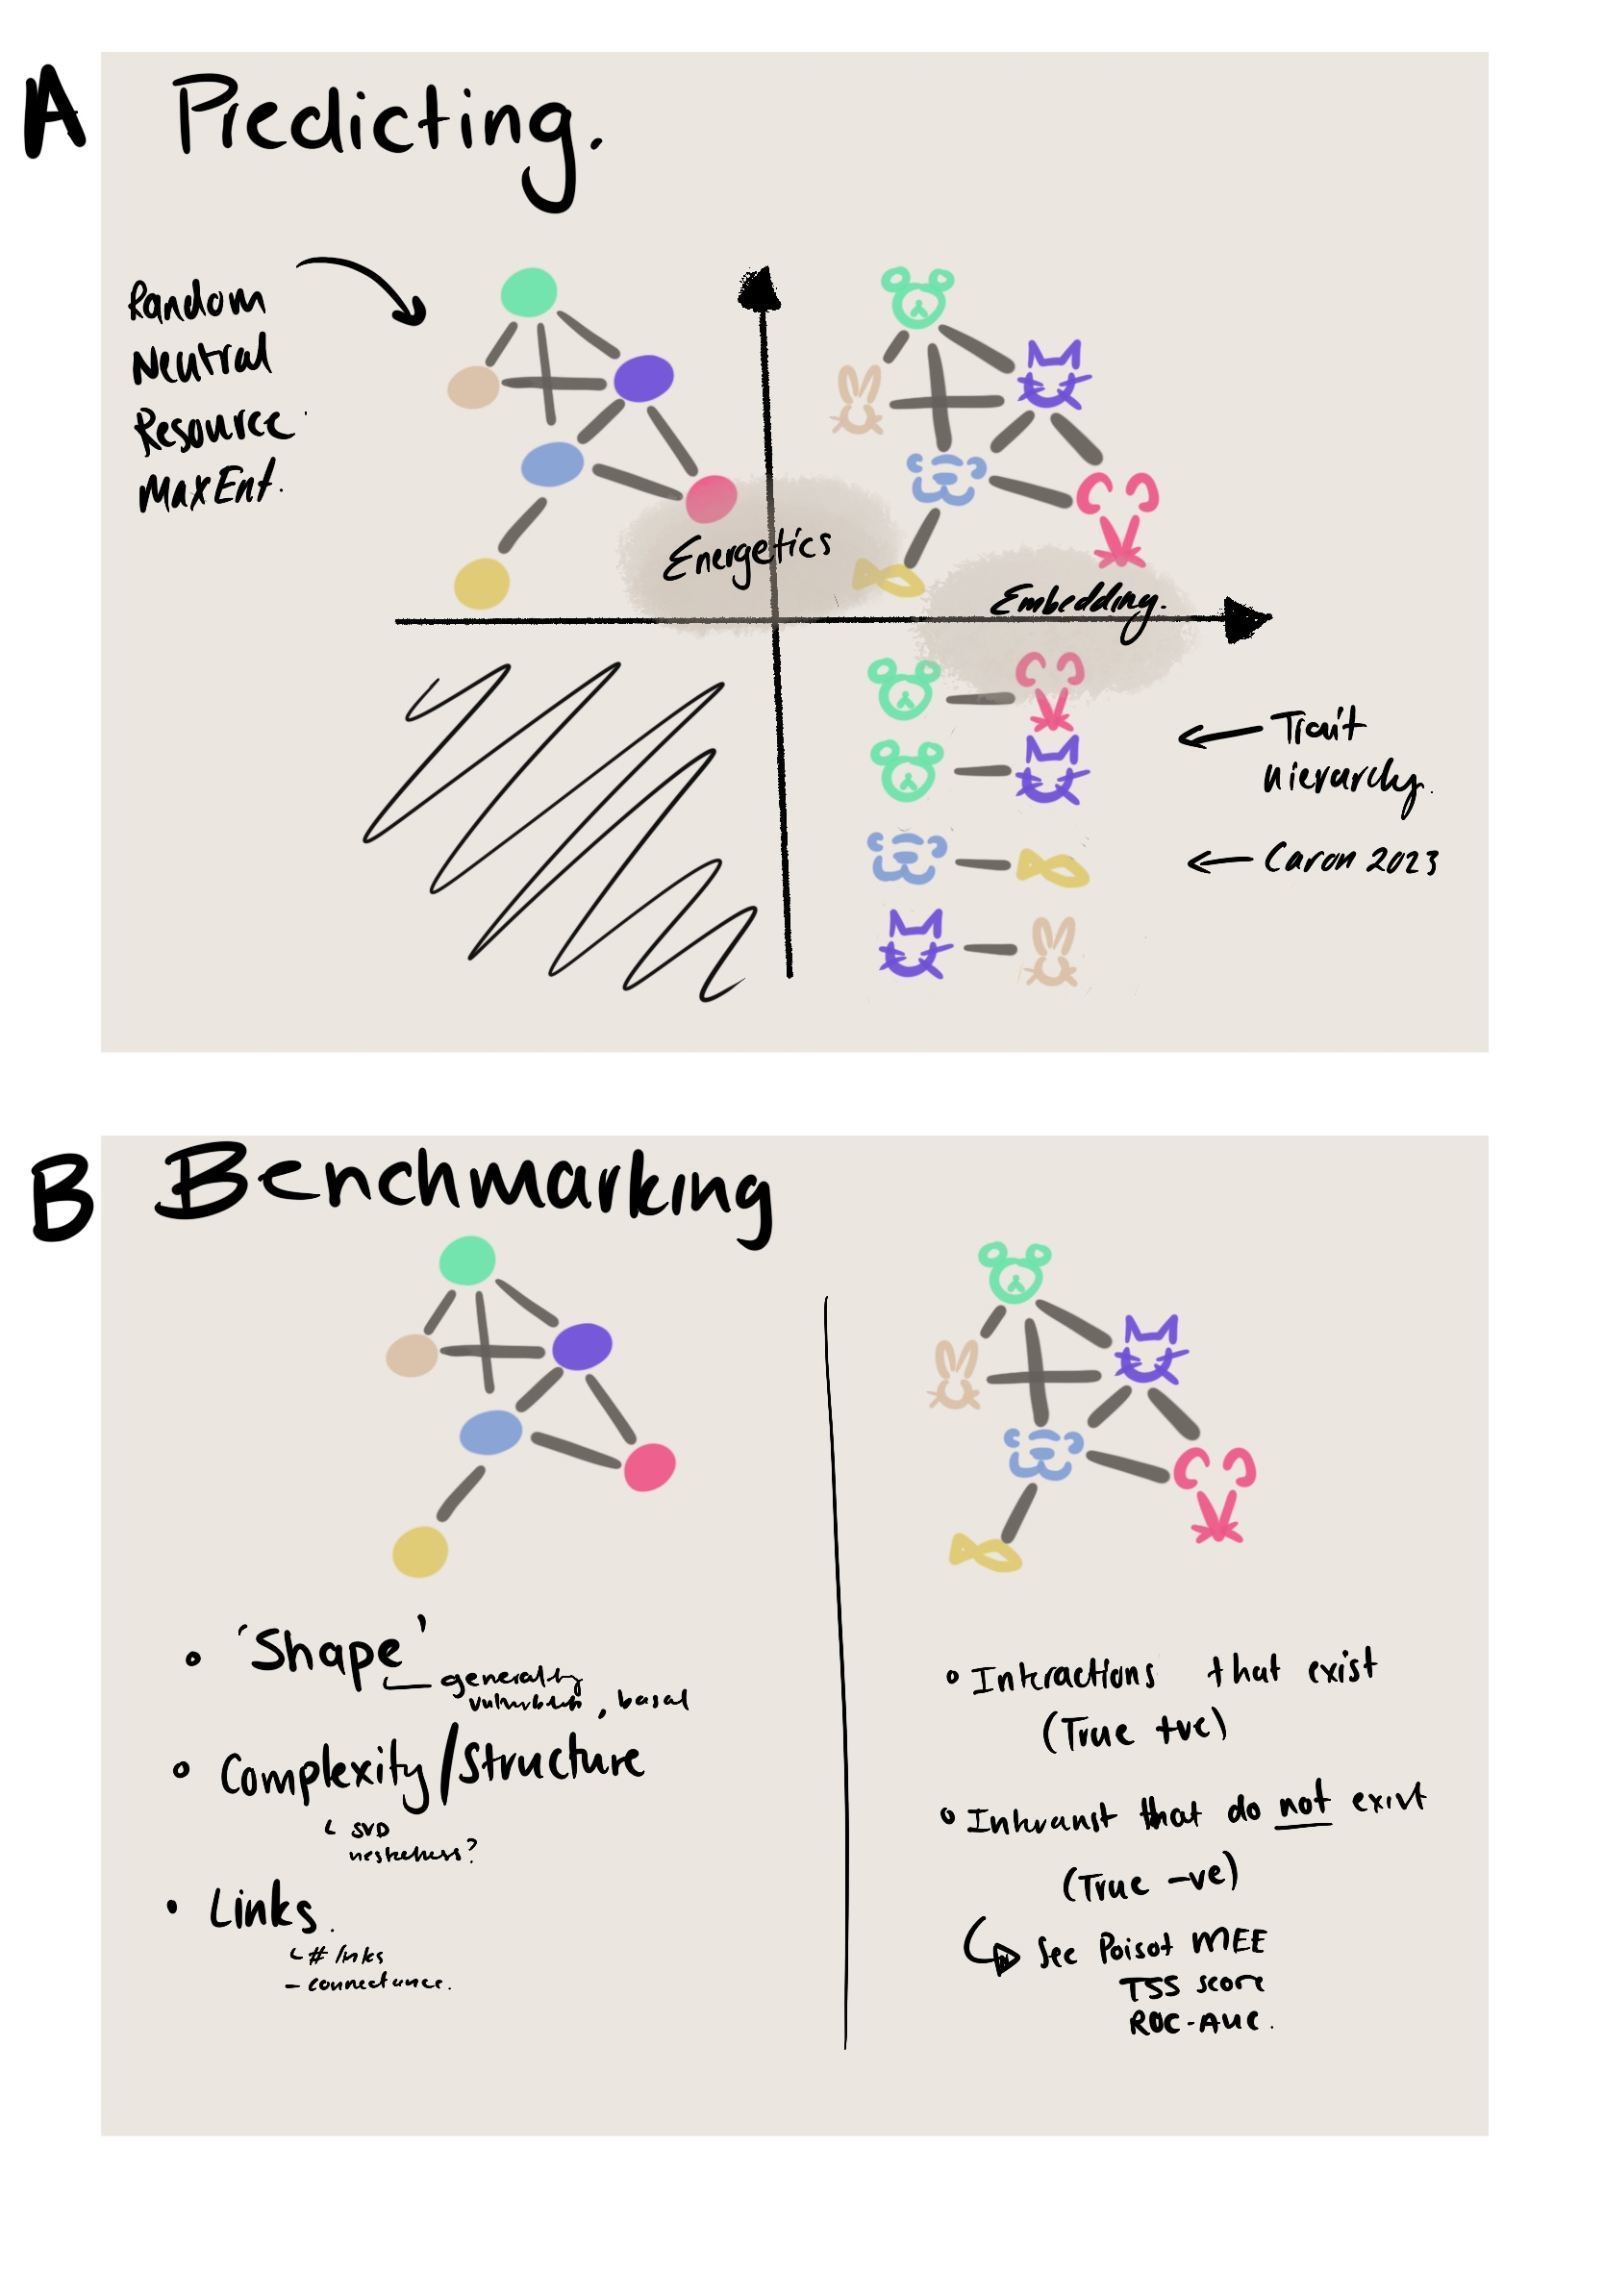
\includegraphics{images/concept.jpeg}

}

\caption{\label{fig-concept}Conceptual figure of the `network
prediction'. Panel A shows where the model families fall in the the
context of being models that predict networks or models that predict
interactions space. Panel B serves to highlight the characteristics one
might like to `test'/benchmark for a model based on it being either a
network or interaction predicting model}

\end{figure}%

\begin{figure}[H]

{\centering 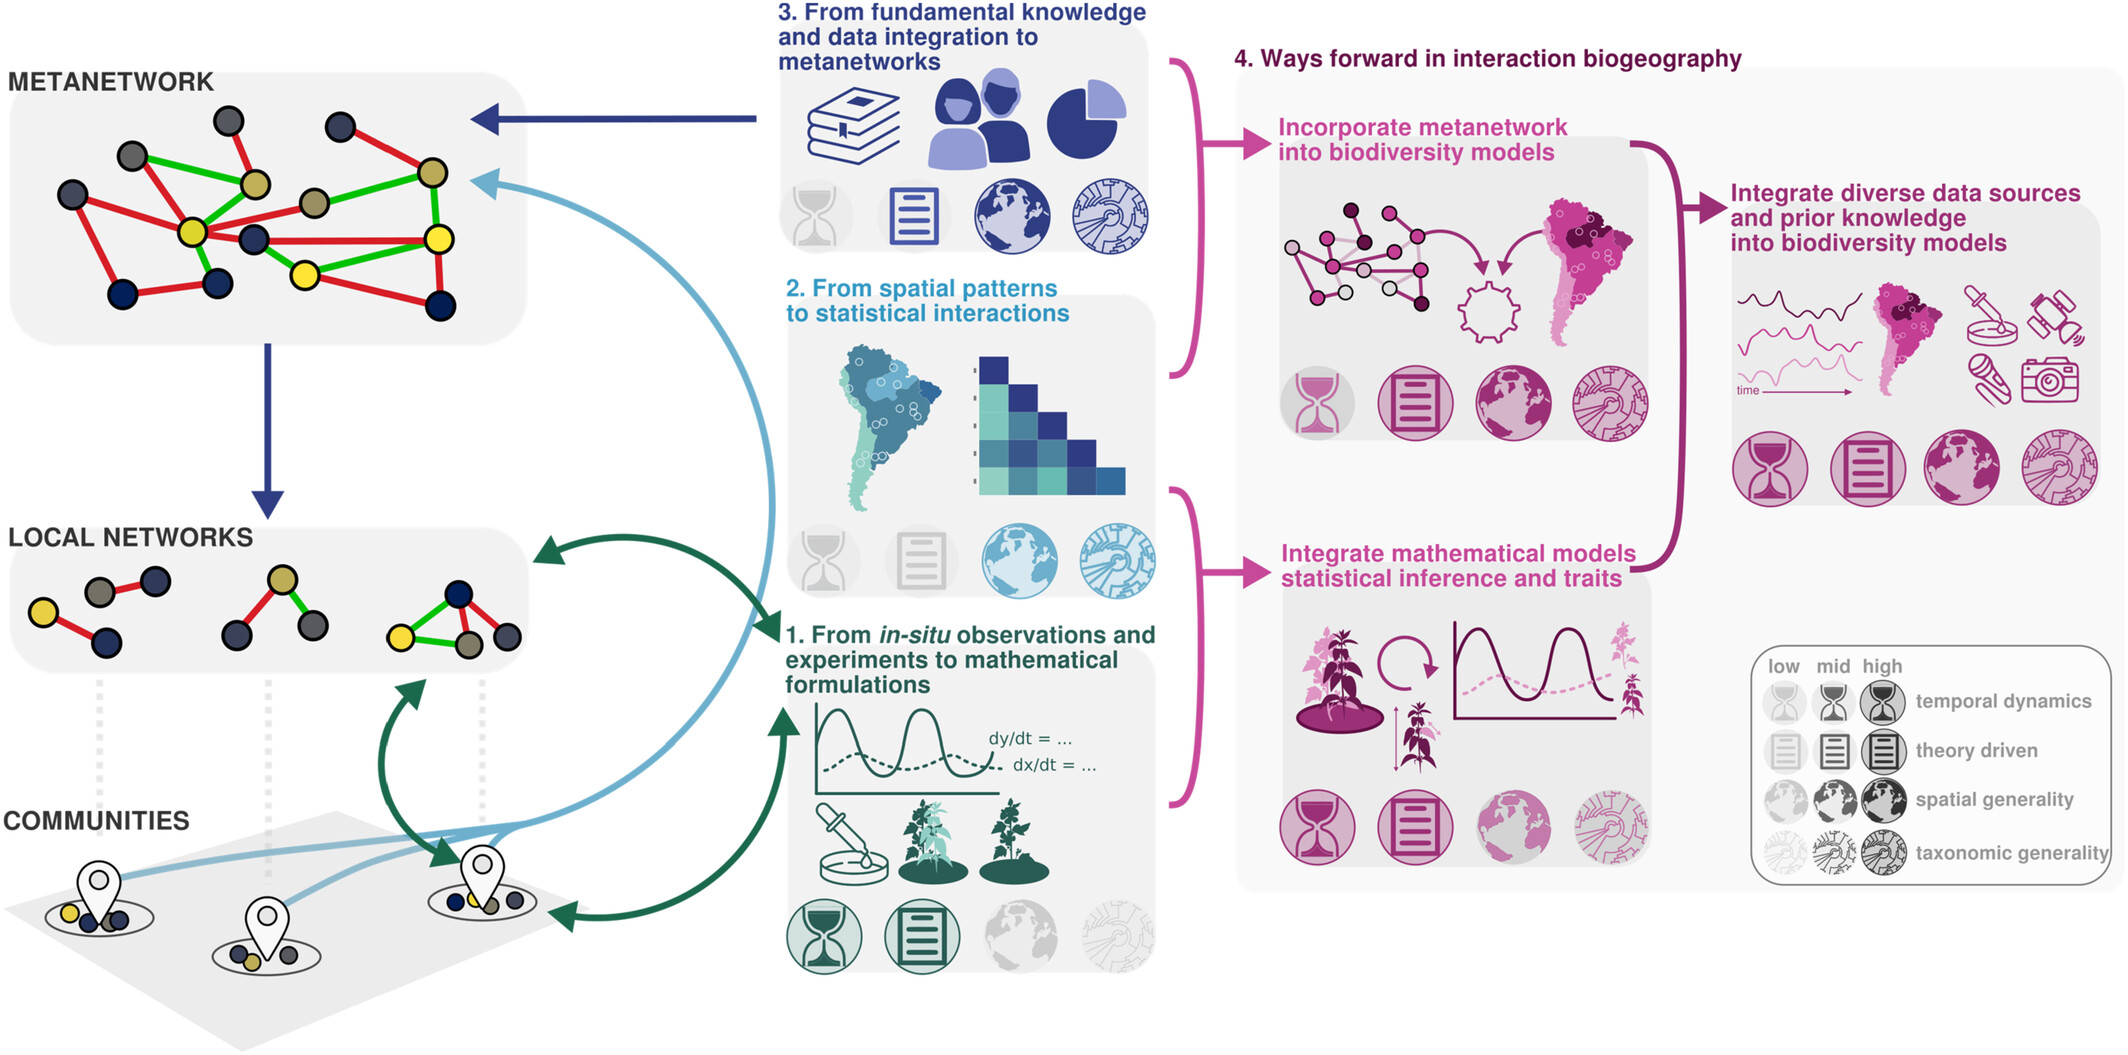
\includegraphics{images/thullier_2023_concept.jpeg}

}

\caption{I like the use of the different source indicator items (not to
dissimilar from Tall Tom's nature paper but also different). This is
from Thuiller et al. (2024)}

\end{figure}%

\textbf{Null models:} The interactions between species occurs regardless
of the identity of the species (\emph{i.e.,} species have no agency) and
links are randomly distributed throughout the network. There is however
the assumption that a network will be constrained by the number of
links. Type I (Fortuna and Bascompte 2006), where interactions happen
proportionally to connectance and Type II (Bascompte et al. 2003), where
interactions happen proportionally to the joint degree of the two
species involved. These two models are equivalent to the Erdos-Renyi and
Configuration models (Newman 2010) respectively (check that though).

\textbf{Neutral models:} Based on the theory that interactions occur as
the result of the abundance of species (\emph{i.e.,} the species still
has no agency but its abundance does?). See Pomeranz et al. (2019)

\textbf{Resource models:} Based on the idea that networks follow a
trophic hierarchy and that species interactions can be determined using
a single dimension {[}the ``niche axis''; Allesina, Alonso, and Pascual
(2008){]}. Essentially these models can be viewed as being based on the
idea of resource partitioning (niches) along a one-dimensional resource
and that the number of links scale with species richness (linear link
scaling). That is, there is some sort of hierarchical feeding based on
how a `resource' is partitioned. Broadly this family consists of three
core models; the cascade model (Joel E. Cohen, Briand, and Newman 1990),
which rests on the idea that species feed on one another in a
hierarchical manner; the niche model (Williams and Martinez 2000),
broadly all species are randomly assigned a `feeding niche' and all
species that fall in this niche can be consumed by that species; and the
nested hierarchy model (Cattin et al. 2004), which adds some component
of phylogenetic clustering/signal\ldots{} so not a single dimension?
\textbf{TODO}. Williams and Martinez (2008) provides a broader overview
of some of the variations in these models as well as comparison between
them regarding their ability to retrieve elements of networks structure
(see also Allesina, Alonso, and Pascual (2008)).

\textbf{Generative models:} (this is maybe a bit of a bold term to use).
MaxEnt (Banville, Gravel, and Poisot 2023), (maybe) stochastic block
(Xie et al. 2017).

\textbf{Feeding models:} Broadly this family of models is rooted in
feeding theory and allocates the links between species based on
energetics, which predicts the diet of a consumer based on energy
intake. This means that the model is focused on predicting not only the
number of links in a network but also the arrangement of these links
based on the diet breadth of a species. The diet breadth model
(Beckerman, Petchey, and Warren 2006) as well as its allometrically
scaled cousin the allometric diet breadth model (ADBM) (Petchey et al.
2008) determine links between species based on the energetic content,
handling time, and density of species. See also DeAngelis, Goldstein,
and O'Neill (1975)

\begin{quote}
Gravel et al. (2013) also poses an interesting cross-over between the
adbm and niche model.
\end{quote}

\textbf{Binary classifiers:} The task of predicting if an interaction
will occur between a species pair is treated as a statistical binary
classification task, where the task is to correlate `real world'
interaction data with a suitable ecological proxy for which data is more
widely available (\emph{e.g.,} traits). Model families often used
include generalised linear models (\emph{e.g.,} Caron et al. 2022),
random forest (\emph{e.g.,} Llewelyn et al. 2023), trait-based k-NN
(\emph{e.g.,} Desjardins-Proulx et al. 2017), and Bayesian models
(\emph{e.g.,} Eklöf, Tang, and Allesina 2013; Cirtwill et al. 2019). See
Pichler et al. (2020) for a more detailed overview on the performance of
machine learning and statistical approaches for inferring trait-trait
relationships.

\textbf{Graph embedding:} This family of approaches has been extensively
discussed in Strydom et al. (2023) but can be broadly explained as an
approach that estimates latent features from observed networks that can
be used to predict interactions. Strydom et al. (2022) uses a transfer
learning framework (specifically using a random dot product graph for
embedding) based around the idea that interactions are evolutionarily
conserved and that we can use known networks, and phylogenetic
relationships, to predict interactions for a given species pool.
\textbf{TODO} Log-ratio (Rohr et al. 2010)

\textbf{Trait matching:} Interactions are determined by a series of
`feeding rules', whereby the interaction between a species pair will
only occur if all feeding rules are met. These rules are determined on
an \emph{a priori} basis using expert/ecological knowledge to determine
the underlying feeding hierarchy using ecological proxies
(Morales-Castilla et al. 2015). For example the Paleo Foodweb Inference
Model (PFIM, Shaw et al. 2024) uses a series of rules for a set of trait
categories (such as habitat and body size) to determine if an
interaction can occur between a species pair. What sets this family of
models apart from \textbf{expert knowledge} ones is that there is a
formalisation of the feeding rules and thus there is some ability to
transfer these rules to different communities.

\textbf{Expert knowledge:} Not so much about empirical observations but
more the value of `local' knowledge and having specific individuals
sitting around a table and assigning a value of how confident they are
that a specific species pair are likely to interact (\emph{e.g.,}
Jennifer A. Dunne et al. 2008), this has the added advantage that
interactions can be scored in a more categorical as opposed to binary
fashion, \emph{e.g.,} Maiorano et al. (2020) score interactions as
either obligate (typical food resources) or occasional (opportunistic
feeding) interactions. I feel like its worth also mentioning downfalls
\emph{a la} Brimacombe et al. (2023)\ldots{}

\textbf{Data scavenging:} There are also a lot of published
\emph{interaction} data that are publicly available \emph{e.g.,} the
Global Biotic Interactions (GloBI) database (Poelen, Simons, and Mungall
2014) and these can also be used to construct an interaction network by
mining these sources to look for interactions for specific species
pairs. This is done by matching species pairs against those within a
dataset of trophic interactions to determine if an interaction is
present or absent between the two species (\emph{e.g.,} the WebBuilder
tool developed by Gray et al. 2015). It is important to note that this
methodology is only going to be able to infer observations that have
been recorded in the field, and given the relative scarcity {[}\emph{I
say Poisot et al. (2021) but that's more an overview of complete
networks but one can also get pairwise interactions from these types of
data so I feel like its okay?}{]} and localised sampling of these types
of datasets it is very likely that there will be many false negatives
(missing pairwise interactions) using this approach.

\section{Model benchmarking}\label{model-benchmarking}

\begin{itemize}
\item
  `Testing' the performance of a model is going to depend on some of the
  core limitations of the model itself thus it makes sense to think of
  two sets benchmarking rules for network and interaction prediction
  models respectively (see Figure~\ref{fig-concept} panel B).
\item
  When it comes to network models we are concerned with the
  `preservation' of structure and distribution of links across the
  network. For interaction models we want to ensure that we are able to
  retrieve interactions that really exist but also those that cannot
  exist (\emph{sensu} forbidden links Jordano (2016b))
\end{itemize}

\begin{quote}
``As long as these predictions are not perfect, some interactions will
be predicted at the `wrong' position in the network; these measures
cannot describe the structural effect of these mistakes. On the other
hand, measures of network structure can have the same value with
interactions that fall at drastically different positions; this is in
part because a lot of these measures covary with connectance, and in
part because as long as these values are not 0 or their respective
maximum, there is a large number of network configurations that can have
the same value.'' - Poisot (2023)
\end{quote}

\subsection{Benchmarking network
models}\label{benchmarking-network-models}

\begin{itemize}
\item
  Maybe look at some of the historic papers that compare some of the
  `resource models'
\item
  See also Allesina, Alonso, and Pascual (2008) and the likelihood
  function that they use for model selection
\item
  Look at Vermaat, Dunne, and Gilbert (2009)
\end{itemize}

\begin{quote}
``Possibly, the most striking caveat of the use of summary statistics is
that it cannot tell us whether or not a model is able to fully replicate
empirical networks.'' - Allesina, Alonso, and Pascual (2008)
\end{quote}

\subsection{Benchmarking interaction
models}\label{benchmarking-interaction-models}

\begin{itemize}
\item
  Main concern with predicting interactions is that we want to test the
  `quality' of the links we are predicting (both true positives and true
  negatives), but the inherit sparsity (meaning high class imbalance)
  means that we also need to look at the balance of these predictions.
\item
  ``Both precision and recall may be useful in cases where there is
  imbalanced data. However, it may be valuable to prioritize one over
  the other in cases where the outcome of a false positive or false
  negative is costly.''
\item
  Caveat regarding the use of real world interaction data both for
  training and validating predictions? \emph{e.g.,} Poisot, Ouellet, et
  al.~et al 2021 and Catchen et al 2023
\item
  See Poisot (2023)

  \begin{itemize}
  \item
    skill (ability to make the right prediction; evaluate whether low
    prevalence can lull us into a false sense of predictive accuracy)
  \item
    bias (trends towards systematically over-predicting one class)
  \item
    class imbalance (the relative number of cases representing
    interactions)
  \end{itemize}
\item
  ``These results suggest that learning from a dataset with very low
  connectance can be a different task than for more connected networks:
  it becomes increasingly important to capture the mechanisms that make
  an interaction exist, and therefore having a slightly more biased
  training dataset might be beneficial. As connectance increases, the
  need for biased training sets is less prominent, as learning the rules
  for which interactions do not exist starts gaining importance''
\item
  Maybe also looking at how well a model can recover `missing links'
  \emph{i.e.,} false negatives \emph{sensu} what we did in Strydom et
  al. (2022)
\item
  Need to discuss the key differences and implications between
  predicting a metaweb (\emph{sensu} Jennifer A. Dunne (2006)) and a
  network realisation. Maybe also Poisot, Stouffer, and Gravel (2015)
  that discuss how the local factors are going to play a role.
\end{itemize}

\section{Data \& Methods}\label{sec-data-methods}

\subsection{Selecting models}\label{selecting-models}

This section depends on if we go the family route and where we introduce
them. But a more extended description of each model can be found in the
\texttt{Extended\ Model\ Description} notebook (I'm trying to work out
how to embed this\ldots)

I know tables are awful but in this case they may make more sense. Also
I don't think I'm at the point where I can say that the table is
complete/comprehensive but it getting there Not sure about putting in
some papers that have used the model - totes happy to drop those I
think\ldots{}

\begin{longtable}[]{@{}
  >{\raggedright\arraybackslash}p{(\columnwidth - 14\tabcolsep) * \real{0.1031}}
  >{\raggedright\arraybackslash}p{(\columnwidth - 14\tabcolsep) * \real{0.2062}}
  >{\raggedright\arraybackslash}p{(\columnwidth - 14\tabcolsep) * \real{0.1443}}
  >{\raggedright\arraybackslash}p{(\columnwidth - 14\tabcolsep) * \real{0.0928}}
  >{\raggedright\arraybackslash}p{(\columnwidth - 14\tabcolsep) * \real{0.1546}}
  >{\raggedright\arraybackslash}p{(\columnwidth - 14\tabcolsep) * \real{0.1031}}
  >{\raggedright\arraybackslash}p{(\columnwidth - 14\tabcolsep) * \real{0.0928}}
  >{\raggedright\arraybackslash}p{(\columnwidth - 14\tabcolsep) * \real{0.1031}}@{}}
\caption{Lets make a table that gives an overview of the different model
families and some of their features}\label{tbl-history}\tabularnewline
\toprule\noalign{}
\begin{minipage}[b]{\linewidth}\raggedright
Model family
\end{minipage} & \begin{minipage}[b]{\linewidth}\raggedright
Theory
\end{minipage} & \begin{minipage}[b]{\linewidth}\raggedright
Example used
\end{minipage} & \begin{minipage}[b]{\linewidth}\raggedright
Predicts
\end{minipage} & \begin{minipage}[b]{\linewidth}\raggedright
Needs (minimum)
\end{minipage} & \begin{minipage}[b]{\linewidth}\raggedright
Assembly
\end{minipage} & \begin{minipage}[b]{\linewidth}\raggedright
Constraints
\end{minipage} & \begin{minipage}[b]{\linewidth}\raggedright
Interaction
\end{minipage} \\
\midrule\noalign{}
\endfirsthead
\toprule\noalign{}
\begin{minipage}[b]{\linewidth}\raggedright
Model family
\end{minipage} & \begin{minipage}[b]{\linewidth}\raggedright
Theory
\end{minipage} & \begin{minipage}[b]{\linewidth}\raggedright
Example used
\end{minipage} & \begin{minipage}[b]{\linewidth}\raggedright
Predicts
\end{minipage} & \begin{minipage}[b]{\linewidth}\raggedright
Needs (minimum)
\end{minipage} & \begin{minipage}[b]{\linewidth}\raggedright
Assembly
\end{minipage} & \begin{minipage}[b]{\linewidth}\raggedright
Constraints
\end{minipage} & \begin{minipage}[b]{\linewidth}\raggedright
Interaction
\end{minipage} \\
\midrule\noalign{}
\endhead
\bottomrule\noalign{}
\endlastfoot
null & Network structure is random & & network & network (species
agnostic) & random & link & binary \\
neutral & Network structure is random, but species abundance plays a
role & Pomeranz et al. (2019) & network & abundance, number of links &
mass effect & link & binary \\
resource & Networks are interval, species can be ordered on a `niche
axis' & & network & richness, connectance & `random' & link & binary \\
generative & Networks are determined by their structural features &
Maximum Entropy (Banville, Gravel, and Poisot 2023) & network & network
(species agnostic) & `random' & & binary \\
energetic & Interactions are determined by foraging theory (feeding
links) & ADBM (Petchey et al. 2008) & interactions & body size &
deterministic & & quantitative \\
graph embedding & Interactions can be predicted from the latent traits
of networks & Transfer Learning (Strydom et al. 2022) & interactions &
interactions, phylogenetic tree, list of target species (species pool) &
& & probabilistic \\
trait matching & Interactions can be inferred by a mechanistic
framework/relationships & PFIM (Shaw et al. 2024) & interactions & prior
(expert) knowledge of trait hierarchy/relationships, traits, list of
target species (species pool) & mechanistic & & \\
binary classifiers & Interactions can be predicted by learning the
relationship between interactions and ecologically relevant predictors &
& interactions & interactions, traits, list of target species (species
pool) & statistical & & \\
expert knowledge & `Boots on the ground' ecological knowledge and
observations & & interactions & list of target species (species pool) &
mechanistic & & \\
data scavenging & Webscraping to create networks from online databases &
& interactions & list of target species (species pool) & & & \\
\end{longtable}

\subsection{Datasets used}\label{datasets-used}

\subsubsection{Mangal networks}\label{mangal-networks}

We queried the Mangal (Poisot et al. 2016) database and extracted a
total of \textbf{TODO} networks. \emph{Some sort of summary as to the
geographic/taxonomic range??} Although these networks represent a high
volume of interaction data they do not have accompanying `metadata' that
we would need for some of the more data-hungry model families
(\emph{e.g.,} local abundance), the Mangal networks were used to provide
the `starting values' for the random, resource, and generative families.
This allows us to generate a large number of different networks that we
can use to compare and contrast the performance of the various model
families (see Section~\ref{sec-model-benchmarking} for a more detailed
breakdown). For each network from Mangal we generated \textbf{TODO}
versions of that network using each model family.

\begin{quote}
``These complex food webs differ in their level of resolution and
sampling effort, which may introduce noise in the estimation of their
properties, especially given their large number of interacting elements.
However, because our MaxEnt models are applied on imperfect data, they
aim at reproducing the sampled structure of food webs, not their actual
structure.'' - Banville, Gravel, and Poisot (2023) (something to think
about\ldots)
\end{quote}

\subsubsection{Empirical networks}\label{empirical-networks}

`Elite' number of datasets for interaction models

Although the availability of empirical interaction data is growing as
techniques begin to improve and grow (Pringle and Hutchinson 2020), we
still lack a way to define what is the `ideal' interaction dataset.

New Zealand dataset(s): Pomeranz et al. (2019)

\begin{quote}
Here I think we need to span a variety of domains, at minimum aquatic
and terrestrial but maybe there should be a `scale' element as well
\emph{i.e.,} a regional and local network. I think there is going to be
a `turning point' where structural will take over from mechanistic in
terms of performance. More specifically at local scales bioenergetic
constraints (and co-occurrence) may play a bigger role in structuring a
network whereas at the metaweb level then mechanistic may make more
(since by default its about who can potentially interact and obviously
not constrained by real-world scenarios) \emph{sensu} Caron et al.
(2024). Although having said that I feel that contradicts the idea of
backbones (\emph{sensu} Bramon Mora (sp?) et al \& Stouffer et al) But
that might be where we get the idea of core \emph{structure} vs
something like linkage density. So core things like trophic level/chain
length will be conserved but connectance might not (I think I understand
what I'm trying to say here)
\end{quote}

I think we should also use the Jennifer A. Dunne et al. (2008) work.
Because 1) it gives the paleo-centric methods their moment in the sun
and 2) I think it also brings up the interesting question of can we use
modern structure to predict past ones?

\subsection{Model benchmarking}\label{sec-model-benchmarking}

For now the (still essentially pending) workflow/associated code can be
found at the following repository
\href{https://github.com/BecksLab/topology_generators}{BecksLab/topology\_generators}.
This will reflect that which is shown in panel \emph{B} of
Figure~\ref{fig-concept}.

\begin{itemize}
\tightlist
\item
  Data `cost' (some methods might need a lot lot of supporting data vs
  something very light weight)
\item
  I think it would be remiss to not also take into consideration
  computational cost
\item
  Something about the network output - I'm acknowledging my biases and
  saying that probabilistic (or \emph{maybe} weighted) links are the way
\end{itemize}

\subsubsection{Network models}\label{network-models}

Want to compare real vs predicted and then get something that looks like
Figure~\ref{fig-topology}

\begin{itemize}
\item
  connectance, nestedness (Bastolla et al., 2009), modularity (Barber,
  2007), asymmetry (Delmas et al., 2018), and Jaccard network
  dissimilarity (Canard et al., 2014)
\item
  \emph{Shape:} do the models construct tall `pencil' vs flat `pancake'
  networks (Beckerman 2024, pers comms), generality/vulnerability, chain
  length (?)
\item
  \emph{Structure:} Predicting `structure' - SVD (Strydom, Dalla Riva,
  and Poisot 2021) but maybe something like nestedness as well (?)
\item
  \emph{Links:} are the number of links preserved (most network
  predicting models are to some extend link constrained but useful to
  see)
\item
  \emph{Motifs:} Staniczenko et al. (2010) uses S1, S2, S4, S5 from
  Stouffer et al. (2007)

  \begin{itemize}
  \item
    S1: Number of linear chains
  \item
    S2: Number of omnivory motifs
  \item
    S4: Number of apparent competition motifs
  \item
    S5: Number of direct competition motifs
  \end{itemize}
\end{itemize}

\subsubsection{Interaction models}\label{interaction-models}

\begin{itemize}
\tightlist
\item
  Based on Poisot (2023):

  \begin{itemize}
  \tightlist
  \item
    Precision-Recall (PR-AUC) - performance
  \item
    Matthews correlation coefficient (MCC) - accuracy
  \end{itemize}
\item
  Maybe same measures we use for the network models
\end{itemize}

\subsubsection{PVA (action plan)}\label{pva-action-plan}

\begin{enumerate}
\def\labelenumi{\arabic{enumi}.}
\tightlist
\item
  Shortlist/finalise the different topo generators
\item
  collate/translate into \texttt{Julia}

  \begin{itemize}
  \tightlist
  \item
    \emph{e.g.,} some models wil be in SpeciesInteractionNetworks.jl
    (new EcoNet); I know (parts of) the transfer learning stuff is and
    the niche model
  \item
    others will need to be coded out (the more simpler models should be
    easier)
  \end{itemize}
\item
  Curate networks for the different datasets/scenarios we select - I
  feel like there might be some scenarios that we can't do all models
  for all datasets but maybe I'm being a pessimist.

  \begin{itemize}
  \tightlist
  \item
    Need to also think about where one might find the additional data
    for some of the models\ldots{}

    \begin{itemize}
    \tightlist
    \item
      Body size: Herberstein et al. (2022) - Although maybe Andrew has
      strong thotsTM RE the one true body size database to rule them
      all\ldots{}
    \item
      Other trait sources: Wilman et al. (2014) and Jones et al. (2009)
    \item
      This is where we'll get the paleo traits from if I'm correct
      Bambach, Bush, and Erwin (2007)
    \item
      Phylogeny stuff: Upham, Esselstyn, and Jetz (2019) (what we used
      for TL but its only mammals\ldots) but I'm sure there will be
      others
    \end{itemize}
  \item
    Also limitation of scope\ldots{} \emph{e.g.,} do we even dare to
    think about including plants/basal producers (see \emph{e.g.,}
    Valdovinos et al. (2023))
  \item
    Taxonomic harmonisation - something to think about and check
  \end{itemize}
\end{enumerate}

\section{Results}\label{results}

Joel E. Cohen, Newman, and Steele (1985) actually tells us that the
cascade model only really works for communities that range from 3-33
species\ldots{} and Williams and Martinez (2008) also highlights how
structural models really only work for small communities

\subsection{Qualitative stuff}\label{qualitative-stuff}

Maybe not the best term to use but thinking here about practical
limitations of the different families. This can include thinking about:

\begin{itemize}
\tightlist
\item
  scale limitations (time or space); \emph{e.g.,} a metaweb is going to
  encapsulate but not distinguish between different seasons or locations
\item
  data needed. I think this can be in the form of real world datasets
  (\emph{e.g.,} traits) but also \emph{a priori} knowledge (\emph{e.g.,}
  having to define the constraints of a niche model)
\item
  computational costs
\end{itemize}

\begin{figure}[H]

{\centering 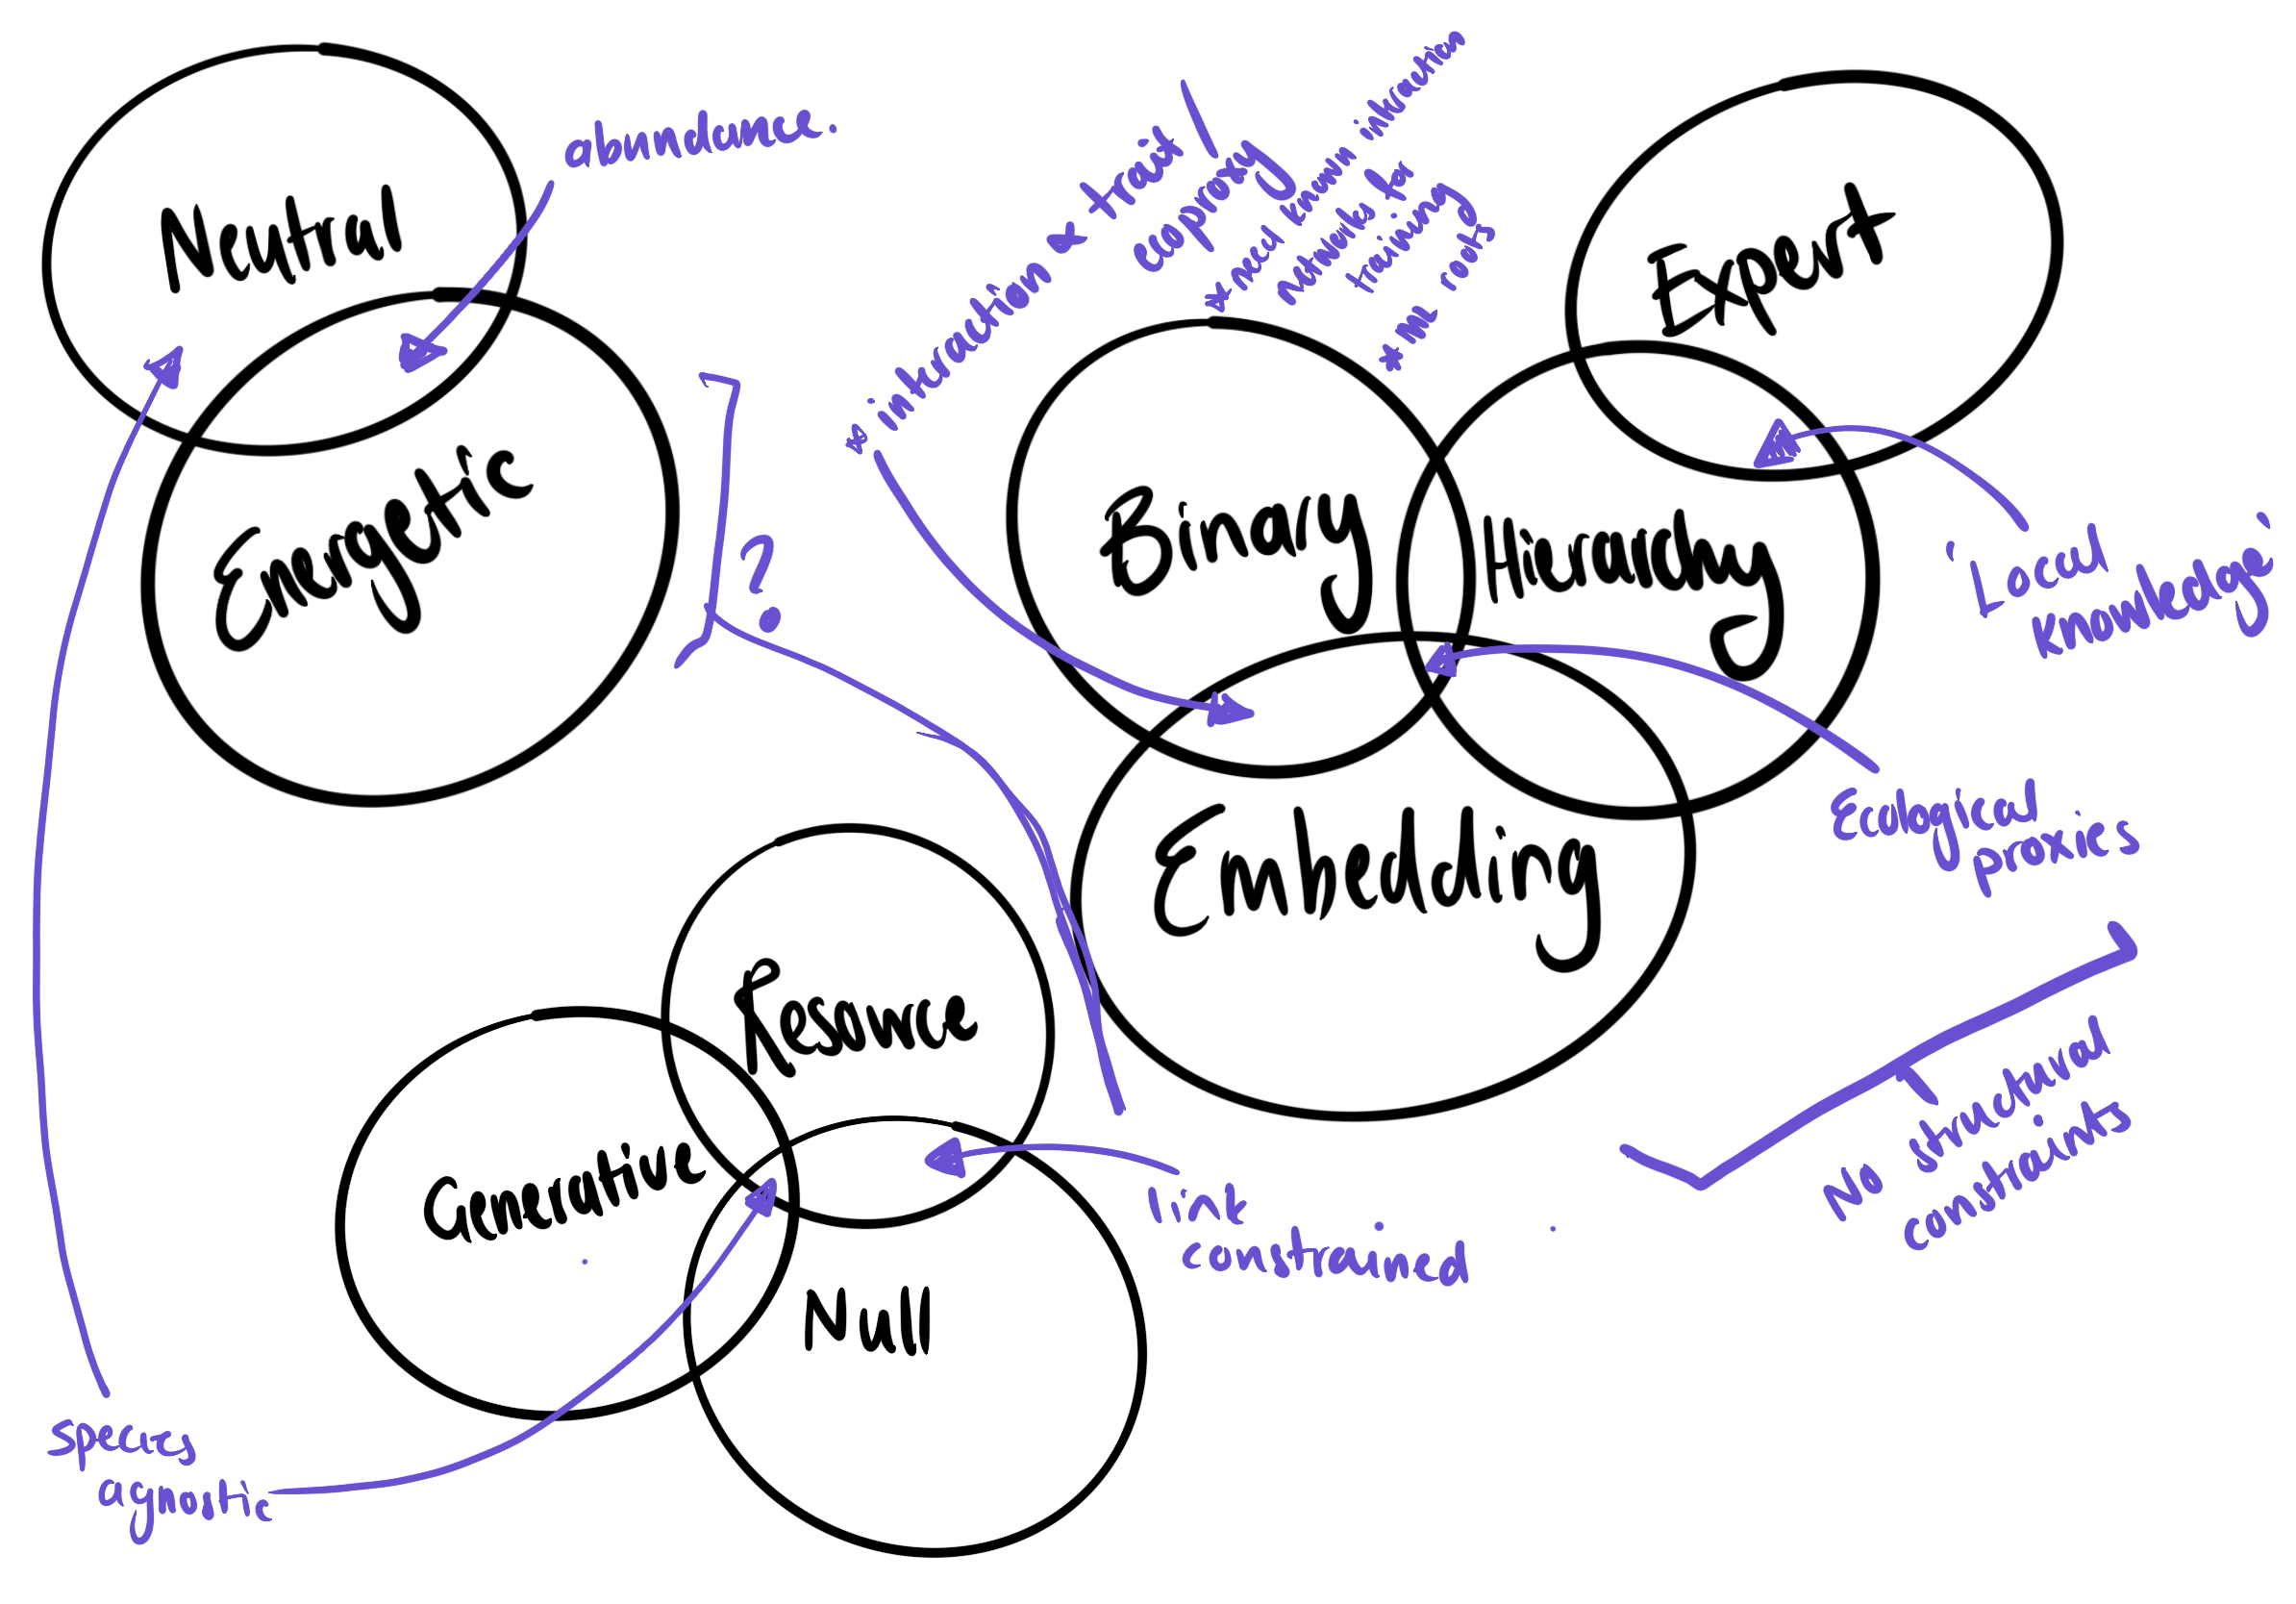
\includegraphics{images/model_venn.png}

}

\caption{I still haven't given up on a sort of venn diagram idea but
maybe it going to be more of a venn-flow chart hybrid\ldots{}}

\end{figure}%

\subsection{Quantitative stuff}\label{quantitative-stuff}

\begin{figure}[H]

\centering{

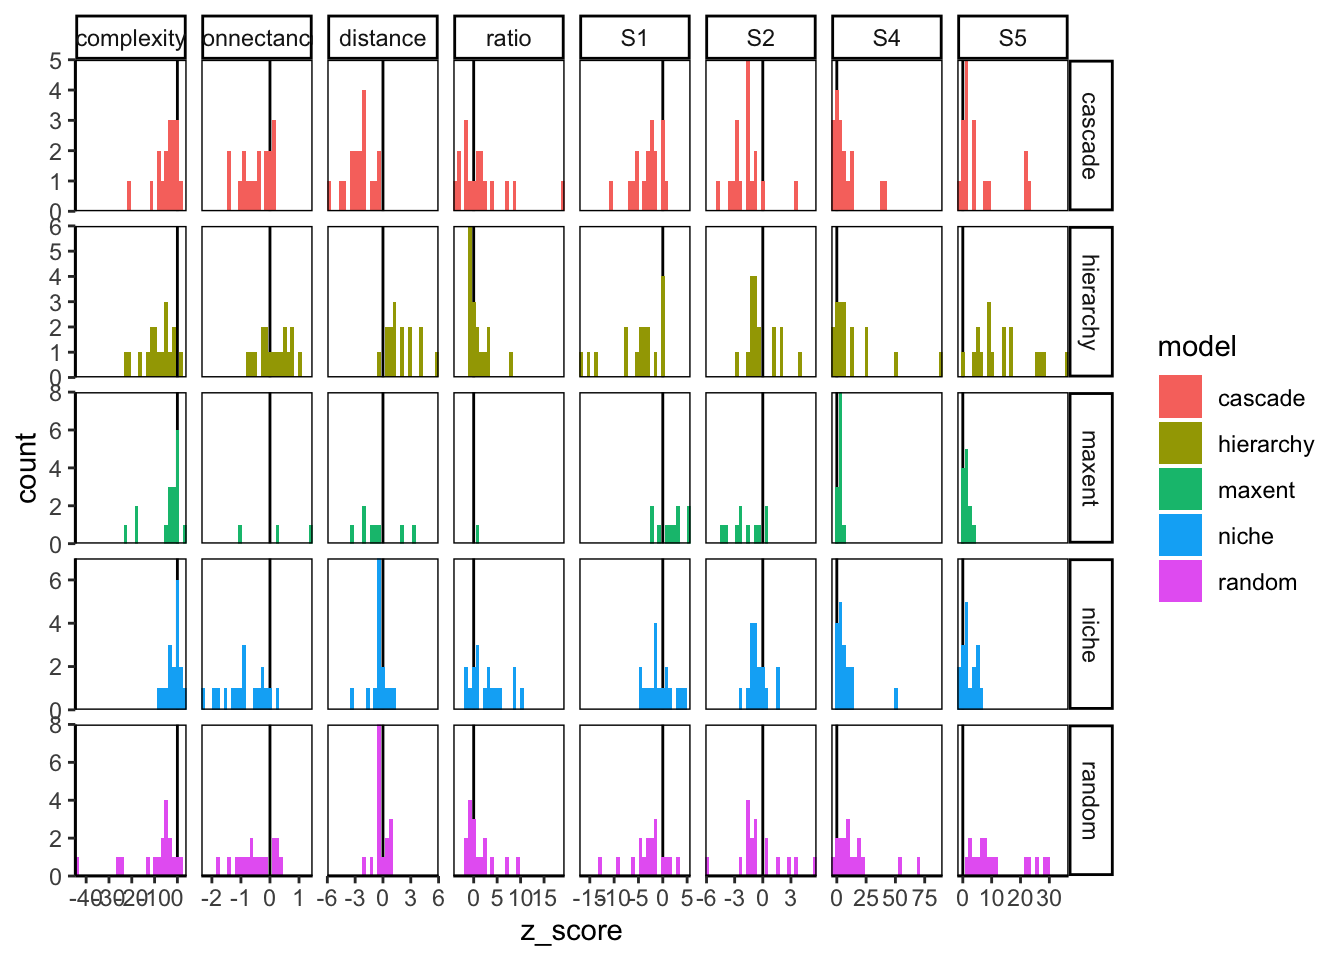
\includegraphics{index_files/figure-latex/notebooks-model_quantitative-fig-topology-output-2.png}

}

\caption{\label{fig-topology}DIfference between real and model network
property. S1 - S5 represent the different motif structures identified in
Stouffer et al. (2007).}

\end{figure}%

\textsubscript{Source:
\href{https://BecksLab.github.io/ms_t_is_for_topology/index.qmd.html}{Article
Notebook}}

I really like this way of plotting results from Pichler et al. (2020)

\begin{figure}

\centering{

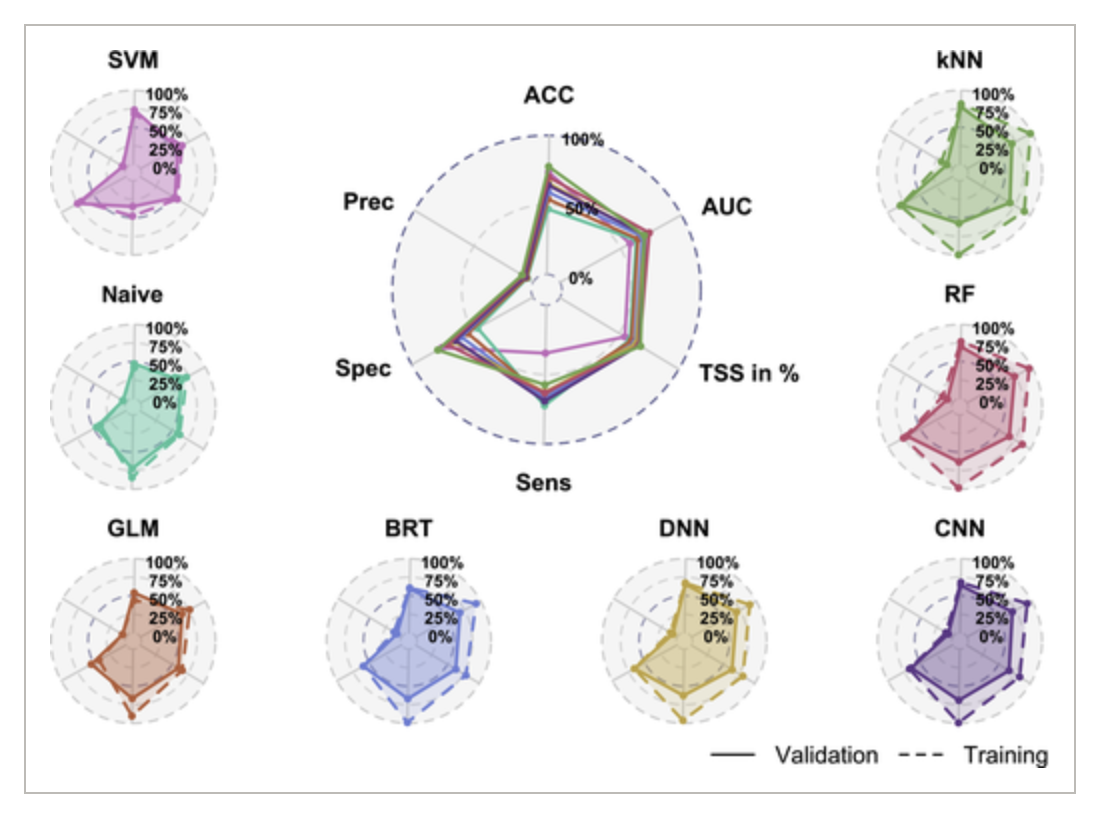
\includegraphics{images/pichler_result.png}

}

\caption{\label{fig-pichler}Cool way to conceptualise results from
Pichler et al. (2020)}

\end{figure}%

\section{Discussion}\label{discussion}

\begin{itemize}
\item
  I think a big take home will (hopefully) be how different approaches
  do better in different situations and so you as an end user need to
  take this into consideration and pick accordingly. I think Petchey et
  al. (2011) might have (and share) some thoughts on this (thanks
  Andrew). I feel like I need to look at Berlow, Brose, and Martinez
  (2008) but maybe not exactly in this context but vaguely adjacent.
\item
  An interesting thing to also think about (and arguably it will be
  addressed based on some of the other thoughts and ideas) is data
  dependant and data independent `parametrisation' of the models\ldots{}
\item
  Why do interaction models do so badly at predicting structure? Nuance
  of metaweb vs realisation but also time? At the core of it interaction
  models are trained on existing interaction data; this is data that are
  most likely closer to a metaweb than a local realisation even if they
  are being inventoried at a small scale.

  \begin{itemize}
  \tightlist
  \item
    I think this is sort of the crux of the argument presented in
    Brimacombe, Bodner, and Fortin (2024)
  \end{itemize}
\end{itemize}

\begin{quote}
\emph{``we highlight an interesting paradox: the models with the best
performance measures are not necessarily the models with the closest
reconstructed network structure.''} - Poisot (2023)
\end{quote}

\begin{itemize}
\item
  \emph{Do we need network models to predict interactions and
  interaction models to predict structure?} (lets not think about that
  too hard or I might just have to sit in silence for a while\ldots)

  \begin{itemize}
  \tightlist
  \item
    ``Another argument for the joint prediction of networks and
    interactions is to reduce circularity and biases in the predictions.
    As an example, models like linear filtering generate probabilities
    of non-observed interactions existing, but do so based on measured
    network properties.'' - Strydom et al. (2021)
  \end{itemize}
\item
  It will be interesting to bring up the idea that if a model is missing
  a specific pairwise link but doing well at the structural level then
  when does it matter?
\item
  Close out with a call to action that we have models that predict
  networks very well and models that predict interactions very well but
  nothing that is doing well at predicting both - this is where we
  should be focusing our attention when it comes to furthering model
  development. (we need models that will fill the space in the top right
  quadrant of panel A in Figure~\ref{fig-concept})
\end{itemize}

\section*{References}\label{references}
\addcontentsline{toc}{section}{References}

\textsubscript{Source:
\href{https://BecksLab.github.io/ms_t_is_for_topology/index.qmd.html}{Article
Notebook}}

\phantomsection\label{refs}
\begin{CSLReferences}{1}{0}
\bibitem[\citeproctext]{ref-allesinaGeneralModelFood2008}
Allesina, Stefano, David Alonso, and Mercedes Pascual. 2008. {``A
{General Model} for {Food Web Structure}.''} \emph{Science} 320 (5876):
658--61. \url{https://doi.org/10.1126/science.1156269}.

\bibitem[\citeproctext]{ref-bambachAutecologyFillingEcospace2007}
Bambach, Richard K., Andrew M. Bush, and Douglas H. Erwin. 2007.
{``Autecology and the {Filling} of {Ecospace}: {Key Metazoan
Radiations}.''} \emph{Palaeontology} 50 (1): 1--22.
\url{https://doi.org/10.1111/j.1475-4983.2006.00611.x}.

\bibitem[\citeproctext]{ref-banvilleWhatConstrainsFood2023}
Banville, Francis, Dominique Gravel, and Timothée Poisot. 2023. {``What
Constrains Food Webs? {A} Maximum Entropy Framework for Predicting Their
Structure with Minimal Biases.''} \emph{PLOS Computational Biology} 19
(9): e1011458. \url{https://doi.org/10.1371/journal.pcbi.1011458}.

\bibitem[\citeproctext]{ref-bascompteNestedAssemblyPlantanimal2003}
Bascompte, J., P. Jordano, C. J. Melian, and J. M. Olesen. 2003. {``The
Nested Assembly of Plant-Animal Mutualistic Networks.''}
\emph{Proceedings of the National Academy of Sciences} 100 (16):
9383--87. \url{https://doi.org/10.1073/pnas.1633576100}.

\bibitem[\citeproctext]{ref-beckermanForagingBiologyPredicts2006}
Beckerman, Andrew P., Owen L. Petchey, and Philip H. Warren. 2006.
{``Foraging Biology Predicts Food Web Complexity.''} \emph{Proceedings
of the National Academy of Sciences} 103 (37): 13745--49.
\url{https://doi.org/10.1073/pnas.0603039103}.

\bibitem[\citeproctext]{ref-berlowGoldilocksFactorFood2008}
Berlow, Eric L., Ulrich Brose, and Neo D. Martinez. 2008. {``The
{`{Goldilocks} Factor'} in Food Webs.''} \emph{Proceedings of the
National Academy of Sciences} 105 (11): 4079--80.
\url{https://doi.org/10.1073/pnas.0800967105}.

\bibitem[\citeproctext]{ref-brimacombeApplyingMethodIts2024}
Brimacombe, Chris, Korryn Bodner, and Marie-Josee Fortin. 2024.
{``Applying a Method Before Its Proof-of-Concept: {A} Cautionary Tale
Using Inferred Food Webs.''}
\url{https://doi.org/10.13140/RG.2.2.22076.65927}.

\bibitem[\citeproctext]{ref-brimacombeShortcomingsReusingSpecies2023}
Brimacombe, Chris, Korryn Bodner, Matthew Michalska-Smith, Timothée
Poisot, and Marie-Josée Fortin. 2023. {``Shortcomings of Reusing Species
Interaction Networks Created by Different Sets of Researchers.''}
\emph{PLOS Biology} 21 (4): e3002068.
\url{https://doi.org/10.1371/journal.pbio.3002068}.

\bibitem[\citeproctext]{ref-caronTraitmatchingModelsPredict2024}
Caron, Dominique, Ulrich Brose, Miguel Lurgi, F. Guillaume Blanchet,
Dominique Gravel, and Laura J. Pollock. 2024. {``Trait-Matching Models
Predict Pairwise Interactions Across Regions, Not Food Web
Properties.''} \emph{Global Ecology and Biogeography} 33 (4): e13807.
\url{https://doi.org/10.1111/geb.13807}.

\bibitem[\citeproctext]{ref-caronAddressingEltonianShortfall2022}
Caron, Dominique, Luigi Maiorano, Wilfried Thuiller, and Laura J.
Pollock. 2022. {``Addressing the {Eltonian} Shortfall with Trait-Based
Interaction Models.''} \emph{Ecology Letters} 25 (4): 889--99.
\url{https://doi.org/10.1111/ele.13966}.

\bibitem[\citeproctext]{ref-cattinPhylogeneticConstraintsAdaptation2004}
Cattin, Marie-France, Louis-Félix Bersier, Carolin Banašek-Richter,
Richard Baltensperger, and Jean-Pierre Gabriel. 2004. {``Phylogenetic
Constraints and Adaptation Explain Food-Web Structure.''} \emph{Nature}
427 (6977): 835--39. \url{https://doi.org/10.1038/nature02327}.

\bibitem[\citeproctext]{ref-cirtwillQuantitativeFrameworkInvestigating2019}
Cirtwill, Alyssa R., Anna Eklf, Tomas Roslin, Kate Wootton, and
Dominique Gravel. 2019. {``A Quantitative Framework for Investigating
the Reliability of Empirical Network Construction.''} \emph{Methods in
Ecology and Evolution} 0 (ja).
\url{https://doi.org/10.1111/2041-210X.13180}.

\bibitem[\citeproctext]{ref-cohenCommunityFoodWebs1990}
Cohen, Joel E, Frederic Briand, and Charles Newman. 1990.
\emph{Community {Food Webs}: {Data} and {Theory}}. Biomathematics.
Berlin Heidelberg: Springer-Verlag.

\bibitem[\citeproctext]{ref-cohenStochasticTheoryCommunity1985}
Cohen, Joel E., C. M. Newman, and John Hyslop Steele. 1985. {``A
Stochastic Theory of Community Food Webs {I}. {Models} and Aggregated
Data.''} \emph{Proceedings of the Royal Society of London. Series B.
Biological Sciences} 224 (1237): 421--48.
\url{https://doi.org/10.1098/rspb.1985.0042}.

\bibitem[\citeproctext]{ref-deangelisModelTropicInteraction1975}
DeAngelis, D. L., R. A. Goldstein, and R. V. O'Neill. 1975. {``A {Model}
for {Tropic Interaction}.''} \emph{Ecology} 56 (4): 881--92.
\url{https://doi.org/10.2307/1936298}.

\bibitem[\citeproctext]{ref-desjardins-proulxEcologicalInteractionsNetflix2017}
Desjardins-Proulx, Philippe, Idaline Laigle, Timothée Poisot, and
Dominique Gravel. 2017. {``Ecological Interactions and the {Netflix}
Problem.''} \emph{PeerJ} 5: e3644.
\url{https://doi.org/10.7717/peerj.3644}.

\bibitem[\citeproctext]{ref-dunneNetworkStructureFood2006}
Dunne, Jennifer A. 2006. {``The {Network Structure} of {Food Webs}.''}
In \emph{Ecological Networks: {Linking} Structure and Dynamics}, edited
by Jennifer A Dunne and Mercedes Pascual, 27--86. Oxford University
Press.

\bibitem[\citeproctext]{ref-dunneCompilationNetworkAnalyses2008}
Dunne, Jennifer A., Richard J. Williams, Neo D. Martinez, Rachel A.
Wood, and Douglas H. Erwin. 2008. {``Compilation and {Network Analyses}
of {Cambrian Food Webs}.''} \emph{PLOS Biology} 6 (4): e102.
\url{https://doi.org/10.1371/journal.pbio.0060102}.

\bibitem[\citeproctext]{ref-eklofSecondaryExtinctionsFood2013}
Eklöf, Anna, Si Tang, and Stefano Allesina. 2013. {``Secondary
Extinctions in Food Webs: A {Bayesian} Network Approach.''} Edited by
Jessica Metcalf. \emph{Methods in Ecology and Evolution} 4 (8): 760--70.
\url{https://doi.org/10.1111/2041-210X.12062}.

\bibitem[\citeproctext]{ref-fortunaHabitatLossStructure2006}
Fortuna, Miguel A., and Jordi Bascompte. 2006. {``Habitat Loss and the
Structure of Plant-Animal Mutualistic Networks: {Mutualistic} Networks
and Habitat Loss.''} \emph{Ecology Letters} 9 (3): 281--86.
\url{https://doi.org/10.1111/j.1461-0248.2005.00868.x}.

\bibitem[\citeproctext]{ref-gravelInferringFoodWeb2013}
Gravel, Dominique, Timothée Poisot, Camille Albouy, Laure Velez, and
David Mouillot. 2013. {``Inferring Food Web Structure from
Predator--Prey Body Size Relationships.''} \emph{Methods in Ecology and
Evolution} 4 (11): 1083--90.
\url{https://doi.org/10.1111/2041-210X.12103}.

\bibitem[\citeproctext]{ref-grayJoiningDotsAutomated2015}
Gray, Clare, David H. Figueroa, Lawrence N. Hudson, Athen Ma, Dan
Perkins, and Guy Woodward. 2015. {``Joining the Dots: {An} Automated
Method for Constructing Food Webs from Compendia of Published
Interactions.''} \emph{Food Webs} 5 (December): 11--20.
\url{https://doi.org/10.1016/j.fooweb.2015.09.001}.

\bibitem[\citeproctext]{ref-herbersteinAnimalTraitsCuratedAnimal2022}
Herberstein, Marie E., Donald James McLean, Elizabeth Lowe, Jonas O.
Wolff, Md Kawsar Khan, Kaitlyn Smith, Andrew P. Allen, et al. 2022.
{``{AnimalTraits} - a Curated Animal Trait Database for Body Mass,
Metabolic Rate and Brain Size.''} \emph{Scientific Data} 9 (1): 265.
\url{https://doi.org/10.1038/s41597-022-01364-9}.

\bibitem[\citeproctext]{ref-jonesPanTHERIASpecieslevelDatabase2009}
Jones, Kate E., Jon Bielby, Marcel Cardillo, Susanne A. Fritz, Justin
O'Dell, C. David L. Orme, Kamran Safi, et al. 2009. {``{PanTHERIA}: A
Species-Level Database of Life History, Ecology, and Geography of Extant
and Recently Extinct Mammals.''} \emph{Ecology} 90 (9): 2648--48.
\url{https://doi.org/10.1890/08-1494.1}.

\bibitem[\citeproctext]{ref-jordanoChasingEcologicalInteractions2016}
Jordano, Pedro. 2016a. {``Chasing {Ecological Interactions}.''}
\emph{PLOS Biology} 14 (9): e1002559.
\url{https://doi.org/10.1371/journal.pbio.1002559}.

\bibitem[\citeproctext]{ref-jordanoSamplingNetworksEcological2016}
---------. 2016b. {``Sampling Networks of Ecological Interactions.''}
\emph{Functional Ecology}, September.
\url{https://doi.org/10.1111/1365-2435.12763}.

\bibitem[\citeproctext]{ref-llewelynPredictingPredatorPrey2023}
Llewelyn, John, Giovanni Strona, Christopher R. Dickman, Aaron C.
Greenville, Glenda M. Wardle, Michael S. Y. Lee, Seamus Doherty, Farzin
Shabani, Frédérik Saltré, and Corey J. A. Bradshaw. 2023. {``Predicting
Predator--Prey Interactions in Terrestrial Endotherms Using Random
Forest.''} \emph{Ecography} 2023 (9): e06619.
\url{https://doi.org/10.1111/ecog.06619}.

\bibitem[\citeproctext]{ref-maioranoTETRAEUSpecieslevelTrophic2020}
Maiorano, Luigi, Alessandro Montemaggiori, Gentile Francesco Ficetola,
Louise O'Connor, and Wilfried Thuiller. 2020. {``{TETRA-EU} 1.0: {A}
Species-Level Trophic Metaweb of {European} Tetrapods.''} \emph{Global
Ecology and Biogeography} 29 (9): 1452--57.
\url{https://doi.org/10.1111/geb.13138}.

\bibitem[\citeproctext]{ref-morales-castillaInferringBioticInteractions2015}
Morales-Castilla, Ignacio, Miguel G. Matias, Dominique Gravel, and
Miguel B. Araújo. 2015. {``Inferring Biotic Interactions from
Proxies.''} \emph{Trends in Ecology \& Evolution} 30 (6): 347--56.
\url{https://doi.org/10.1016/j.tree.2015.03.014}.

\bibitem[\citeproctext]{ref-newmanNetworksIntroduction2010}
Newman, Mark E. J. 2010. \emph{Networks. {An} Introduction}. New York,
NY: Oxford University Press.

\bibitem[\citeproctext]{ref-petcheySizeForagingFood2008}
Petchey, Owen L., Andrew P. Beckerman, Jens O. Riede, and Philip H.
Warren. 2008. {``Size, Foraging, and Food Web Structure.''}
\emph{Proceedings of the National Academy of Sciences} 105 (11):
4191--96. \url{https://doi.org/10.1073/pnas.0710672105}.

\bibitem[\citeproctext]{ref-petcheyFitEfficiencyBiology2011}
---------. 2011. {``Fit, Efficiency, and Biology: {Some} Thoughts on
Judging Food Web Models.''} \emph{Journal of Theoretical Biology} 279
(1): 169--71. \url{https://doi.org/10.1016/j.jtbi.2011.03.019}.

\bibitem[\citeproctext]{ref-pichlerMachineLearningAlgorithms2020}
Pichler, Maximilian, Virginie Boreux, Alexandra-Maria Klein, Matthias
Schleuning, and Florian Hartig. 2020. {``Machine Learning Algorithms to
Infer Trait-Matching and Predict Species Interactions in Ecological
Networks.''} \emph{Methods in Ecology and Evolution} 11 (2): 281--93.
\url{https://doi.org/10.1111/2041-210X.13329}.

\bibitem[\citeproctext]{ref-poelenGlobalBioticInteractions2014}
Poelen, Jorrit H., James D. Simons, and Chris J. Mungall. 2014.
{``Global Biotic Interactions: {An} Open Infrastructure to Share and
Analyze Species-Interaction Datasets.''} \emph{Ecological Informatics}
24 (November): 148--59.
\url{https://doi.org/10.1016/j.ecoinf.2014.08.005}.

\bibitem[\citeproctext]{ref-poisotGuidelinesPredictionSpecies2023}
Poisot, Timothée. 2023. {``Guidelines for the Prediction of Species
Interactions Through Binary Classification.''} \emph{Methods in Ecology
and Evolution} 14 (5): 1333--45.
\url{https://doi.org/10.1111/2041-210X.14071}.

\bibitem[\citeproctext]{ref-poisotMangalMakingEcological2016}
Poisot, Timothée, Benjamin Baiser, Jennifer Dunne, Sonia Kéfi, François
Massol, Nicolas Mouquet, Tamara N. Romanuk, Daniel B. Stouffer, Spencer
A. Wood, and Dominique Gravel. 2016. {``Mangal -- Making Ecological
Network Analysis Simple.''} \emph{Ecography} 39 (4): 384--90.
\url{https://doi.org/10.1111/ecog.00976}.

\bibitem[\citeproctext]{ref-poisotGlobalKnowledgeGaps2021}
Poisot, Timothée, Gabriel Bergeron, Kevin Cazelles, Tad Dallas,
Dominique Gravel, Andrew MacDonald, Benjamin Mercier, Clément Violet,
and Steve Vissault. 2021. {``Global Knowledge Gaps in Species
Interaction Networks Data.''} \emph{Journal of Biogeography} n/a (n/a).
\url{https://doi.org/10.1111/jbi.14127}.

\bibitem[\citeproctext]{ref-poisotSpeciesWhyEcological2015}
Poisot, Timothée, Daniel B. Stouffer, and Dominique Gravel. 2015.
{``Beyond Species: Why Ecological Interaction Networks Vary Through
Space and Time.''} \emph{Oikos} 124 (3): 243--51.
\url{https://doi.org/10.1111/oik.01719}.

\bibitem[\citeproctext]{ref-poisotDescribeUnderstandPredict2016}
Poisot, Timothée, Daniel B. Stouffer, and Sonia Kéfi. 2016. {``Describe,
Understand and Predict: Why Do We Need Networks in Ecology?''}
\emph{Functional Ecology} 30 (12): 1878--82.
\url{https://www.jstor.org/stable/48582345}.

\bibitem[\citeproctext]{ref-pomeranzInferringPredatorPrey2019}
Pomeranz, Justin P. F., Ross M. Thompson, Timothée Poisot, and Jon S.
Harding. 2019. {``Inferring Predator--Prey Interactions in Food Webs.''}
\emph{Methods in Ecology and Evolution} 10 (3): 356--67.
\url{https://doi.org/10.1111/2041-210X.13125}.

\bibitem[\citeproctext]{ref-pringleUntanglingFoodWebs2020}
Pringle, Robert M. 2020. {``Untangling {Food Webs}.''} In
\emph{Untangling {Food Webs}}, 225--38. Princeton University Press.
\url{https://doi.org/10.1515/9780691195322-020}.

\bibitem[\citeproctext]{ref-pringleResolvingFoodWebStructure2020}
Pringle, Robert M., and Matthew C. Hutchinson. 2020. {``Resolving
{Food-Web Structure}.''} \emph{Annual Review of Ecology, Evolution and
Systematics} 51 (Volume 51, 2020): 55--80.
\url{https://doi.org/10.1146/annurev-ecolsys-110218-024908}.

\bibitem[\citeproctext]{ref-rohrModelingFoodWebs2010}
Rohr, Rudolf Philippe, Heike Scherer, Patrik Kehrli, Christian Mazza,
and Louis-Félix Bersier. 2010. {``Modeling {Food Webs}: {Exploring
Unexplained Structure Using Latent Traits}.''} \emph{The American
Naturalist} 176 (2): 170--77. \url{https://doi.org/10.1086/653667}.

\bibitem[\citeproctext]{ref-shawFrameworkReconstructingAncient2024}
Shaw, Jack O., Alexander M. Dunhill, Andrew P. Beckerman, Jennifer A.
Dunne, and Pincelli M. Hull. 2024. {``A Framework for Reconstructing
Ancient Food Webs Using Functional Trait Data.''} bioRxiv.
\url{https://doi.org/10.1101/2024.01.30.578036}.

\bibitem[\citeproctext]{ref-staniczenkoStructuralDynamicsRobustness2010}
Staniczenko, Phillip P. A., Owen T. Lewis, Nick S. Jones, and Felix
Reed-Tsochas. 2010. {``Structural Dynamics and Robustness of Food
Webs.''} \emph{Ecology Letters} 13 (7): 891--99.
\url{https://doi.org/10.1111/j.1461-0248.2010.01485.x}.

\bibitem[\citeproctext]{ref-stoufferEvidenceExistenceRobust2007}
Stouffer, Daniel B, Juan Camacho, Wenxin Jiang, and Luís A Nunes Amaral.
2007. {``Evidence for the Existence of a Robust Pattern of Prey
Selection in Food Webs.''} \emph{Proceedings of the Royal Society B:
Biological Sciences} 274 (1621): 1931--40.
\url{https://doi.org/10.1098/rspb.2007.0571}.

\bibitem[\citeproctext]{ref-strydomFoodWebReconstruction2022}
Strydom, Tanya, Salomé Bouskila, Francis Banville, Ceres Barros,
Dominique Caron, Maxwell J. Farrell, Marie-Josée Fortin, et al. 2022.
{``Food Web Reconstruction Through Phylogenetic Transfer of Low-Rank
Network Representation.''} \emph{Methods in Ecology and Evolution} 13
(12): 2838--49. \url{https://doi.org/10.1111/2041-210X.13835}.

\bibitem[\citeproctext]{ref-strydomGraphEmbeddingTransfer2023}
Strydom, Tanya, Salomé Bouskila, Francis Banville, Ceres Barros,
Dominique Caron, Maxwell J. Farrell, Marie-Josée Fortin, et al. 2023.
{``Graph Embedding and Transfer Learning Can Help Predict Potential
Species Interaction Networks Despite Data Limitations.''} \emph{Methods
in Ecology and Evolution} 14 (12): 2917--30.
\url{https://doi.org/10.1111/2041-210X.14228}.

\bibitem[\citeproctext]{ref-strydomRoadmapPredictingSpecies2021}
Strydom, Tanya, Michael D. Catchen, Francis Banville, Dominique Caron,
Gabriel Dansereau, Philippe Desjardins-Proulx, Norma R. Forero-Muñoz, et
al. 2021. {``A Roadmap Towards Predicting Species Interaction Networks
(Across Space and Time).''} \emph{Philosophical Transactions of the
Royal Society B: Biological Sciences} 376 (1837): 20210063.
\url{https://doi.org/10.1098/rstb.2021.0063}.

\bibitem[\citeproctext]{ref-strydomSVDEntropyReveals2021}
Strydom, Tanya, Giulio V. Dalla Riva, and Timothée Poisot. 2021. {``{SVD
Entropy Reveals} the {High Complexity} of {Ecological Networks}.''}
\emph{Frontiers in Ecology and Evolution} 9.
\url{https://doi.org/10.3389/fevo.2021.623141}.

\bibitem[\citeproctext]{ref-thuillerNavigatingIntegrationBiotic2024}
Thuiller, Wilfried, Irene Calderón-Sanou, Loïc Chalmandrier, Pierre
Gaüzère, Louise M. J. O'Connor, Marc Ohlmann, Giovanni Poggiato, and
Tamara Münkemüller. 2024. {``Navigating the Integration of Biotic
Interactions in Biogeography.''} \emph{Journal of Biogeography} 51 (4):
550--59. \url{https://doi.org/10.1111/jbi.14734}.

\bibitem[\citeproctext]{ref-uphamInferringMammalTree2019}
Upham, Nathan S., Jacob A. Esselstyn, and Walter Jetz. 2019.
{``Inferring the Mammal Tree: {Species-level} Sets of Phylogenies for
Questions in Ecology, Evolution, and Conservation.''} \emph{PLOS
Biology} 17 (12): e3000494.
\url{https://doi.org/10.1371/journal.pbio.3000494}.

\bibitem[\citeproctext]{ref-valdovinosBioenergeticFrameworkAboveground2023}
Valdovinos, Fernanda S., Kayla R. S. Hale, Sabine Dritz, Paul R. Glaum,
Kevin S. McCann, Sophia M. Simon, Elisa Thébault, William C. Wetzel,
Kate L. Wootton, and Justin D. Yeakel. 2023. {``A Bioenergetic Framework
for Aboveground Terrestrial Food Webs.''} \emph{Trends in Ecology \&
Evolution} 38 (3): 301--12.
\url{https://doi.org/10.1016/j.tree.2022.11.004}.

\bibitem[\citeproctext]{ref-vermaatMajorDimensionsFoodweb2009}
Vermaat, Jan E, Jennifer A Dunne, and Alison J Gilbert. 2009. {``Major
Dimensions in Food-Web Structure Properties.''} \emph{Ecology} 90 (1):
278--82. \url{https://www.ncbi.nlm.nih.gov/pubmed/19294932}.

\bibitem[\citeproctext]{ref-williamsSimpleRulesYield2000}
Williams, Richard J., and Neo D. Martinez. 2000. {``Simple Rules Yield
Complex Food Webs.''} \emph{Nature} 404 (6774): 180--83.
\url{https://doi.org/10.1038/35004572}.

\bibitem[\citeproctext]{ref-williamsSuccessItsLimits2008}
---------. 2008. {``Success and Its Limits Among Structural Models of
Complex Food Webs.''} \emph{Journal of Animal Ecology} 77 (3): 512--19.
\url{https://doi.org/10.1111/j.1365-2656.2008.01362.x}.

\bibitem[\citeproctext]{ref-wilmanEltonTraitsSpecieslevelForaging2014}
Wilman, Hamish, Jonathan Belmaker, Jennifer Simpson, Carolina de la
Rosa, Marcelo M. Rivadeneira, and Walter Jetz. 2014. {``{EltonTraits}
1.0: {Species-level} Foraging Attributes of the World's Birds and
Mammals.''} \emph{Ecology} 95 (7): 2027--27.
\url{https://doi.org/10.1890/13-1917.1}.

\bibitem[\citeproctext]{ref-xieCompletenessCommunityStructure2017}
Xie, Jia-Rong, Pan Zhang, Hai-Feng Zhang, and Bing-Hong Wang. 2017.
{``Completeness of {Community Structure} in {Networks}.''}
\emph{Scientific Reports} 7 (1): 5269.
\url{https://doi.org/10.1038/s41598-017-05585-6}.

\end{CSLReferences}



\end{document}
